\documentclass[10pt,final,journal,twoside, a4paper]{IEEEtran}

% Recommended packages from IEEEtran documentation
\usepackage[utf8]{inputenc}
\usepackage[T1]{fontenc}
\usepackage{siunitx}
\usepackage{bm}
\interdisplaylinepenalty=2500

% Citations
\usepackage{cite}

% Tables with footnotes
\usepackage{threeparttable}

% Tikz - used to draw diagrams
\usepackage{tikz,pgfplots}
\usetikzlibrary{shapes}
\usetikzlibrary{arrows}
\usepackage{pgfplots}
\pgfplotsset{compat=1.3}
\fboxsep=0pt

% Listings
\usepackage{minted}

% References and clickable refs
\usepackage{hyperref}
\usepackage{amsmath}
\usepackage{cleveref}


% Hyphenation for field-specific terms
\hyphenation{eindhoven op-tical net-works semi-conduc-tor}

\title{Cityscapes Segmentation}
\author{
    \IEEEauthorblockN{K.H.W. Stolle}
    \IEEEauthorblockA{k.h.w.stolle@student.tue.nl}
}

\begin{document}

    \maketitle

    \begin{abstract}
        Todo: write me
    \end{abstract}
    \begin{IEEEkeywords}
        Cityscapes, Segmentation, CNN
    \end{IEEEkeywords}

    \section{Introduction}
    The Cityscapes Dataset involves a large number of pictures taken from the front of a car while driving through various cities in Germany \cite{Cordts2016Cityscapes}.

In this paper, a practical solution to the pixel-level semantic labeling task is discussed.
This involves predicting a per-pixel semantic labeling of the image without consiering higher-level object instance or boundary information.

First, a baseline is set using an off-the-shelf architecture for semantic segmentation.
This baseline network is then improved by data augmentation and iterative design, after which this solution is tested.
The results of testing are finally interpreted and discussed.

    \section{Baseline}
    The baseline implementation sets a reference point to improve upon and score our method against.

The architecture U-Net is suitable for semantic segmentation~\cite{RonnebergerFB15}.
It can be used as an off-the-shelf network for performing the task.

Our implementation of the UNet is based on~\cite{GH-Pytorch-UNet2018} with some modifications to run on the target system and handle the input files.

    \section{Method}
    \subsection{Data augmentation}
\label{subsec:data-augmentation}


\subsection{Network architecture}
\label{subsec:network-architecture}

    \section{Results}
    \subsection{Baseline}
Training the baseline U-net on the Cityscapes dataset achieves a maximum IoU-score of 0.45 and a loss of 0.55 after 10 epochs.

\begin{figure}
	\centering
	\begin{tabular}{cc}
		\makecell{
			\includegraphics[width=.45\linewidth]{figures/base-out-gt.png} \\
			Ground Truth 
		} &
		\makecell{
			\includegraphics[width=.45\linewidth]{figures/base-out-1.png} \\
			Epoch 1
		} \\
		\makecell{
			\includegraphics[width=.45\linewidth]{figures/base-out-5.png} \\
			Epoch 5
		} &
		\makecell {
			\includegraphics[width=.45\linewidth]{figures/base-out-10.png} \\
			Epoch 10
		} \\ 
		
	\end{tabular}
	\caption{Output samples of the baseline (U-net) network on a random sample of the validation set}    
	\label{fig:res-out-baseline}
\end{figure}

\Cref{fig:res-out-baseline} shows some output samples of this network for a random sample in the validation set. Notice how the network fails to recognize thin objects such as poles and signs. Some parts of the image, such as the sidewalk, appear noisy even after 10 epochs.

\subsection{Data augmentation}
\begin{figure}
	\centering
	\includegraphics[width=0.9\linewidth]{figures/loss-baseline.png}
	\caption{The loss as a function of the training epoch for the baseline (U-net) network after data augmentation}
	\label{fig:res-loss-baseline}
\end{figure}


\Cref{fig:res-loss-baseline} shows the loss function during the training process. Without much effort, the loss has decreased from $0.55$ to $0.50$

\subsection{Threshold}
\begin{figure}
    \centering
    \begin{tabular}{cc}
        \makecell{
            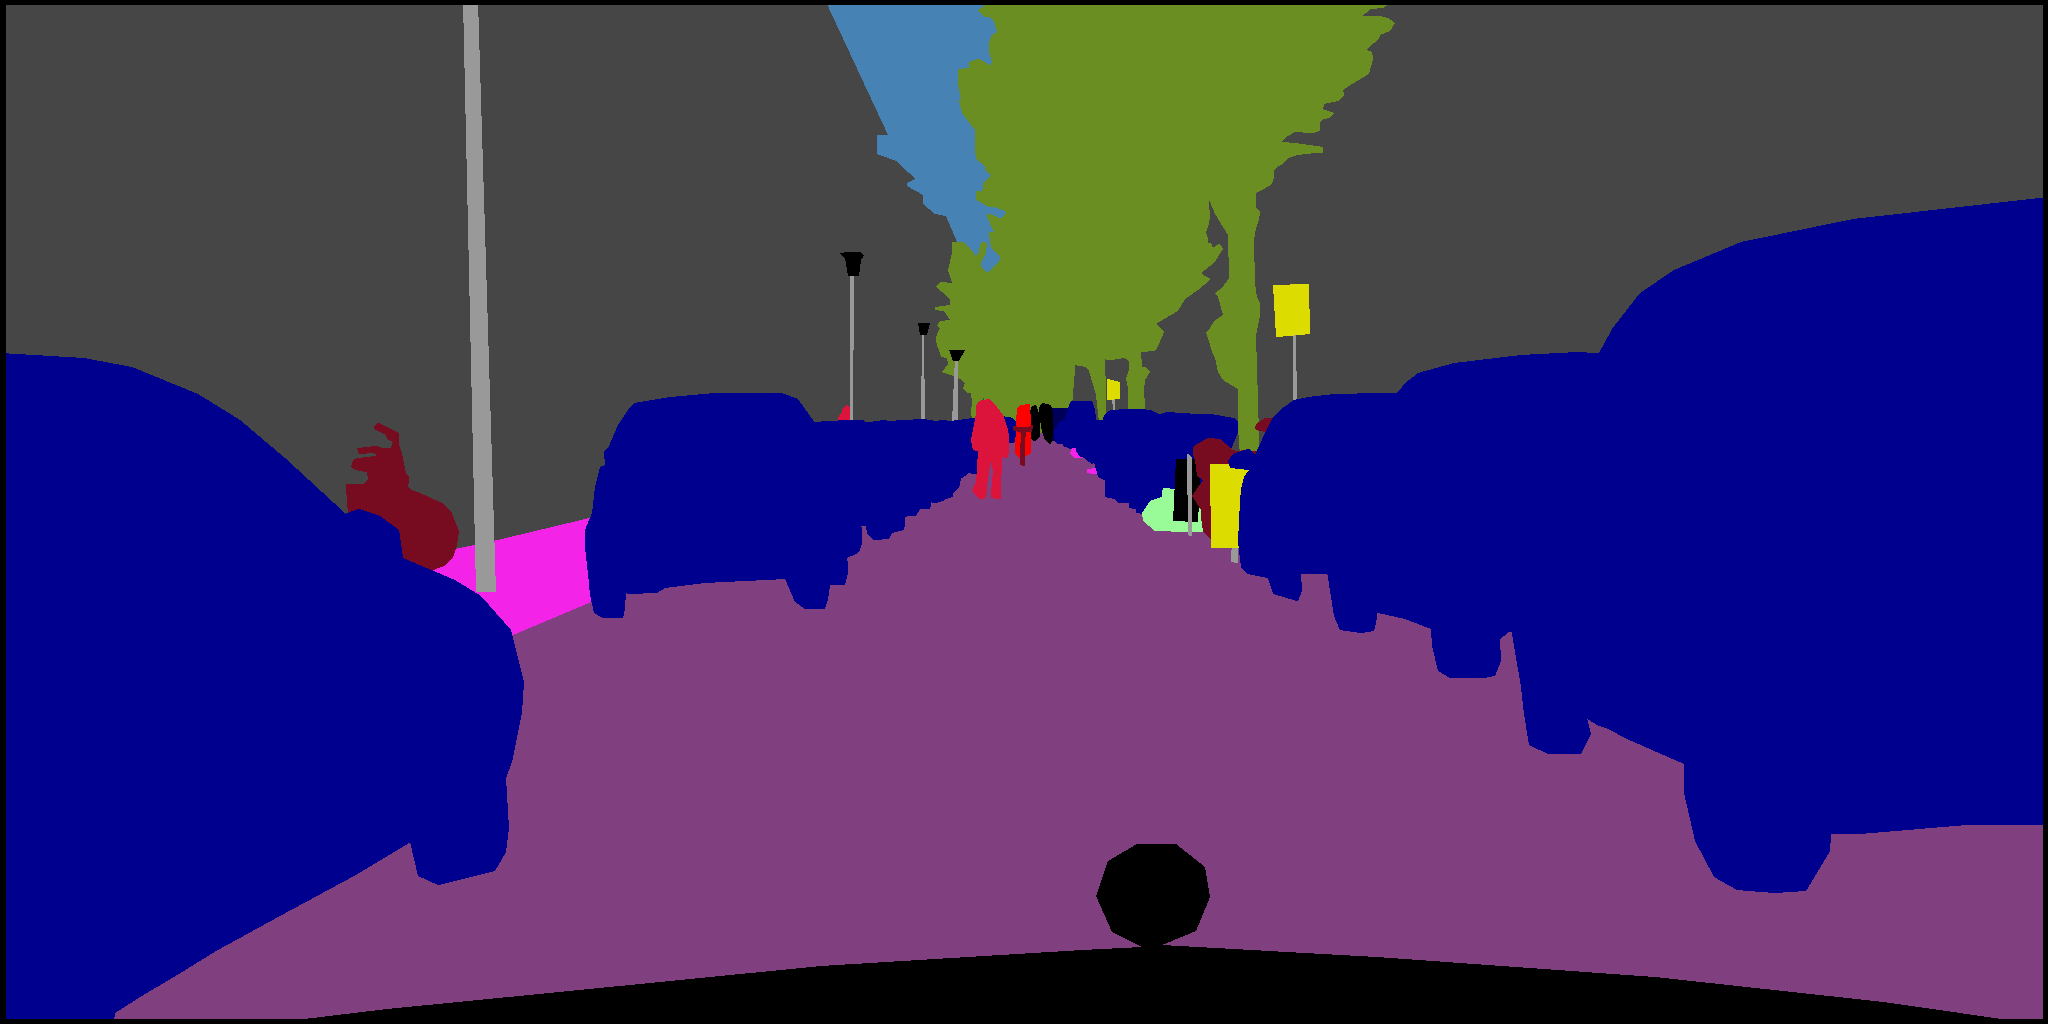
\includegraphics[width=.45\linewidth]{data/threshold/output_truth.png} \\
            Ground Truth 
        } &
        \makecell{
            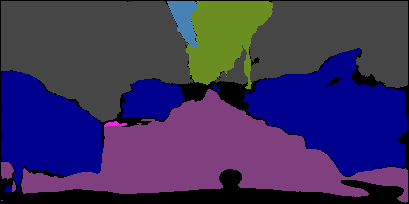
\includegraphics[width=.45\linewidth]{data/threshold/output_1.png} \\
            Epoch 1
        } \\
        \makecell{
            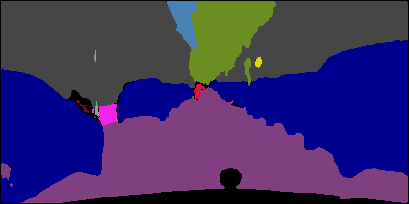
\includegraphics[width=.45\linewidth]{data/threshold/output_5.png} \\
            Epoch 5
        } &
        \makecell {
            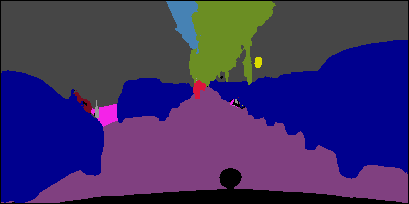
\includegraphics[width=.45\linewidth]{data/threshold/output_10.png} \\
            Epoch 10
        } \\ 
        
    \end{tabular}
    \caption{Ground truth and predicted masks after training for 1, 5 and 10 epochs on a random sample of the validation set using the U-Net model with thresholds and data augmentation}    
    \label{fig:res-out-thres}
\end{figure}

\Cref{fig:res-out-thres} shows the effect of a decision-threshold on the output masks. It appears that the regions with lower confidence, such as at the edges of an object, get ignored sometimes. After 10 epochs, the class masks appear to more closely match the contours of objects.

\begin{figure}
	\centering
	\includegraphics[width=0.9\linewidth]{figures/iou-threshold.png}
	\caption{The IoU as a function of the training epoch for the network with a decision threshold of 0.1.}
	\label{fig:res-iou-thres}
\end{figure}

Notice from \Cref{fig:res-iou-thres} that the IoU now starts at 0 in the untrained network, when all predictions have a confidence less than 0.1. This is to be expected with this method.

Because the decisions of the network do not affect the cross-entropy loss, the loss curve is still exactly the same as in \Cref{fig:res-loss-baseline}. Interestingly, the loss slowly decays while the IoU remains roughly the same after 2 epochs. This can be explained by the nature of loss and decisions: after 2 epochs, predictions are reinforced with a stronger confidence but the classes that hold maximum values that lead to a decision remain roughly the same.

\subsection{Edge detection as input}
\begin{figure}
	\centering
	\subfloat[Loss\label{fig:res-loss-edges}]{
		\centering
		\includegraphics[width=0.45\linewidth]{figures/loss-edges.png}
	}
	\subfloat[IoU\label{fig:res-iou-edges}]{
		\centering
		\includegraphics[width=0.45\linewidth]{figures/iou-edges.png}
	}
	\caption{Loss and IoU as a function of the training epoch for the network with data augmentation, decision threshold and pre-processed edge detection as the 4-th channel of the input image.}
	\label{fig:res-edges}
\end{figure}

\Cref{fig:res-edges} shows the effects of edge detection pre-processing being fed into the network as the 4-th channel. While the loss does not improve significantly, there is a significant improvement of 0.2 for the IoU-score. 

\begin{figure}
	\centering
	\includegraphics[width=0.9\linewidth]{figures/edges-out-10.png}
	\caption{Output of the network with edge detection pre-processing input after 10 epochs.}
	\label{fig:out-edges}
\end{figure}

\cref{fig:out-edges} shows the output of this network after 10 epochs. 
This is the same sample as showcased in \cref{fig:res-out-baseline}. 
By inspection, notice that more fine-details are visible on the output with edge detection, while the logo on the bottom of the car (the black circle) seems to have disappeared.

\subsection{Regularization using dropout}
\begin{figure}
	\centering
	\subfloat[Loss]{
		\centering
		\includegraphics[width=0.45\linewidth]{figures/loss-dropout.png}
	}
	\subfloat[IoU]{
		\centering
		\includegraphics[width=0.45\linewidth]{figures/iou-dropout.png}
	}
	\caption{Loss and IoU as a function of the training epoch for the network with dropout ($p=0.1$) after every convolutional layer.}
	\label{fig:res-dropout}
\end{figure}

\Cref{fig:res-dropout} shows the results with the smallest dropout rate applied. Values between $0.1$ and $0.5$ were tried, but all values had a negative impact on the results. Dropout did thus not positively affect the network and the changes were discarded.

\subsection{Strided convolutions}
\begin{figure}
	\centering
	\subfloat[Loss]{
		\centering
		\includegraphics[width=0.45\linewidth]{figures/loss-stride-in.png}
	}
	\subfloat[IoU]{
		\centering
		\includegraphics[width=0.45\linewidth]{figures/iou-stride-in.png}
	}
	\caption{Loss and IoU as a function of the training epoch with all optimizations enabled and using strided-convolutions to downsample the input}
	\label{fig:res-strided}
\end{figure}
\Cref{fig:res-strided} shows the loss and IoU-score when using strided convolutions to downsample the input. This yields an IoU of 8.4 and a loss of 0.45 after 10 epochs. 

\subsection{Automatic learning rate adjustment}
\begin{figure}
	\centering
	\includegraphics[width=0.9\linewidth]{figures/loss-autolr.png}
	\caption{Loss as a function of the training epoch with all optimizations enabled and automatic learning rate adjustment.}
	\label{fig:res-autolr}
\end{figure}

\Cref{fig:res-autolr} shows the loss with automatic learning rate adjustment. At 2.5 epoch and at 8.5 epoch, the learning rate is adjusted. 
This is evident from the sudden drop in the validation curve. The automatic tuning of the learning rate has no effect on the result of the network, but the solution does appear to converge sooner. 
In order to make the adjustment work, the training process had to be adjusted to validate at more frequent intervals. 
This causes a net slowdown of the learning process. For this reason, this optimization is not part of the final solution.



    \section{Discussion}
    \input{_discussion}

    \section{Conclusion}
    The U-net architecture can be adjusted to perform pixel-level semantic segmentation on the Cityscapes Dataset with a IoU-score of 0.84. To achieve this, the following adjustments were made with respect to the baseline implementation:
\begin{itemize}
	\item Data augmentation
	\item Adding a decision threshold
	\item Pre-processed edge detection as input
	\item Downsampling using strided convolutions
\end{itemize}
\textit{Note that a final score on the test-set was not achieved by the network, as the images had to be compressed too much to be accepted by the Cityscapes testing suite.}

\section{Future work}
The most promising improvement was made by involving edge detection in the network. This was done by feeding a pre-processing step into the network's input. This may not be the optimal solution, as this reduces the amount of features that can be extracted. Another possible solution would be to feed the edge detection into the later layers of the network, after an image is reconstructed by the upsampling layers. Additionally, the edge detection could be also be a learned operation.

A limiting factor in this research was the amount of GPU-memory available. The memory usage of the network could be reduced by applying checkpointing, which trades computation time for memory usage, or by training the network with 16-bit floating point operations instead of 32-bit floating point operations. Future work will have to explore these options.

    \bibliographystyle{IEEEtran}
    \bibliography{library}

\end{document}
